% !TEX root = ../../thesis.tex

\documentclass[../../thesis.tex]{subfiles}
 
\begin{document}

Linear Programming (LP) is a mathematical optimization technique which is used to minimize or maximize 
an objective subject to constraints represented by linear equations. 
If all variables are required to be integers, it is called Integer Programming (IP). 
Integer Programming, in contrast to LP which can be solved efficiently, is often NP-complete.  
Mixed Integer Programming (MIP) takes LP and IP together to form a problem where only some variables 
are required to be integer. MIP problems are also generally NP-complete.

\paragraph{}

The most common MIP problems are of the form:

\begin{align}
  \textrm{min} \quad & \bm{c}^T\bm{x} & \label{mipobj} \\ 
  \textrm{s.t} \quad & A\bm{x} = \bm{b} & \label{miplinearcst} \\
   & \bm{l} \leq \bm{x} \leq \bm{u} & \label{mipboundcst} \\
   & \text{Some or all $x_i$ must take integer values} \label{mipinteger}
\end{align}

(\ref{mipobj}) is the problem objective. $\bm{c}^T$ is the vector of coefficient, $\bm{x}$ is the vector of variables.
(\ref{miplinearcst}) are the linear constraints. $\bm{b}$ is a vector of bounds while $A$ is a matrix of coefficients for the constraints.
(\ref{mipboundcst}) are the bound constraints. Each $x_i$ can only take values between $l_i$ and $u_i$.
And finally, (\ref{mipinteger}) states the integrality constraints over some or all variables.


MIP problems are usually solved using a branch-and-bound algorithm \cite{mip-basics}.
The process is as follows: we start with the MIP formulation and remove all integrality constraints 
to create a resulting linear-programming (LP) relaxation to the original problem. The relaxation can be solved 
easily compared to the original problem. The result might satisfy all integrality constraints and be a solution to the original problem.
But more often than not, a variable has a fractional value.
We can then solve two relaxations by imposing two additional constraints. For example, if $x$ takes value 5.5, we add the 
following linear constraints: $x \leq 5.0$ and $x \geq 6.0$. 
This process is repeated throughout the search tree (\autoref{mip-tree}) a valid solution is found.
More techniques are used to find solutions more efficiently. Each solver uses its
own algorithm (e.g Gurobi Optimizer \cite{mip-basics}).

\begin{figure}
  \centering
  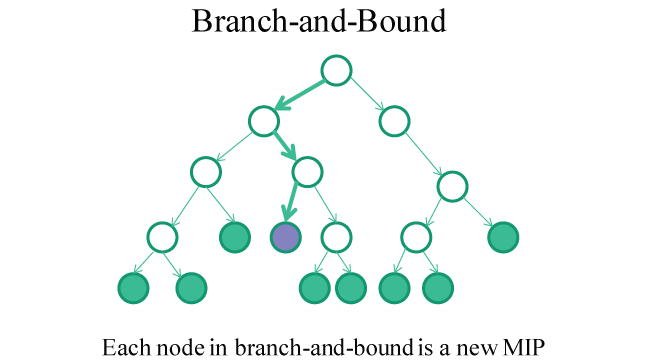
\includegraphics[scale=0.5]{branch-and-bound.png}
  \caption{MIP Branch \& Bound search tree \cite{mip-basics}}
  \label{mip-tree}
\end{figure}

\end{document}

